\chapter{BACKGROUND}
\label{chap:background}

\section{Traditional Statistical Methods for Geographic Assignment}

\subsection{Traditional methods}

The scientific challenge of assigning individuals to their geographic origin based on genetic data predates the current wave of machine learning. Classical approaches were built on population genetics theory, statistical modeling, and multivariate analysis. These methods remain foundational in conservation genetics and wildlife forensics, providing the first rigorous frameworks for linking DNA variation to geography. Four representative approaches—SCAT, SPASIBA, STRUCTURE and KLFDAPC—illustrate the logic behind traditional assignment methods.

\subsubsection{SCAT – Smoothed and Continuous Assignment Tests}

The development of SCAT by Wasser and colleagues (2004) \cite{wasser2004assigning} marked a turning point in applying genetics to wildlife forensics. The core idea of SCAT is to model allele frequencies as continuous surfaces across geographic space rather than discrete population boundaries. By using microsatellite markers from African elephants, SCAT estimated allele frequency gradients through spatial smoothing and then calculated likelihood surfaces for each individual's genotype. This probabilistic framework allowed researchers to infer the most likely geographic origin of ivory samples, even in regions where reference samples were sparse.

The strength of SCAT lies in its ability to interpolate beyond sampled locations, producing continuous assignment maps rather than binary classifications. This was particularly powerful in identifying poaching hotspots in Africa, where many areas lacked dense sampling. Results showed that 50\% of samples were assigned within roughly 500 km of their true origin, and resolution improved substantially in well-sampled regions, sometimes below 200 km. However, the method was computationally intensive, requiring Markov Chain Monte Carlo (MCMC) to approximate posterior distributions, and its accuracy decreased markedly in under-sampled regions. Despite these challenges, SCAT established the feasibility of continuous geographic assignment from limited genetic markers and became a cornerstone for forensic applications.

\subsubsection{SPASIBA – Spatial Bayesian Inference}

Building on the ideas of SCAT, Guillot and colleagues (2016) \cite{guillot2016accurate} developed SPASIBA, a method designed to improve computational efficiency and extend applicability to genome-scale SNP data. SPASIBA treats allele frequencies as spatially autocorrelated random fields, with covariance decaying as geographic distance increases. Instead of relying on MCMC, SPASIBA uses Integrated Nested Laplace Approximation (INLA), a deterministic Bayesian inference method that is far faster and more scalable. This makes it practical to analyze larger datasets with hundreds or thousands of SNPs.

SPASIBA has been applied successfully to a range of taxa, including Florida scrub-jays and \textit{Arabidopsis thaliana}. In the scrub-jay study, using 41 SNPs, SPASIBA localized individuals with a median error of about 26 km, demonstrating impressive resolution at fine scales. In \textit{Arabidopsis}, with 1000 SNPs, the method achieved 75th-percentile errors of around 93 km across the species' European range. These results show that SPASIBA can exploit genome-wide SNP data to generate highly accurate predictions, while also producing probabilistic maps similar to SCAT. Nevertheless, the method assumes Hardy–Weinberg and linkage equilibrium, and like SCAT, its accuracy still depends heavily on reference sampling density. Its computational demands are lower than SCAT's but still non-trivial, requiring specialized software and statistical expertise.

\subsubsection{STRUCTURE – Bayesian Clustering for Population Assignment}

STRUCTURE \cite{pritchard2000inference} implements a Bayesian clustering framework that infers population structure directly from multilocus genotype data without requiring prior knowledge of individual origins. The model assumes Hardy–Weinberg and linkage equilibrium within populations and uses Markov Chain Monte Carlo (MCMC) sampling to assign individuals probabilistically to \textit{K} genetic clusters. Each individual receives a vector of membership coefficients, representing the proportion of its genome originating from each cluster, which allows the detection of both discrete population boundaries and admixture.

In practice, STRUCTURE has been widely applied in conservation genetics to identify distinct populations, measure gene flow, and assign individuals of unknown origin to their most likely population. A critical advantage is its ability to reveal hidden structure: clusters can emerge from the genetic data even when population boundaries are not obvious in the field.

Despite its impact, STRUCTURE has limitations. The method produces clusters rather than explicit spatial coordinates, so its geographic resolution is constrained to population-level inferences. The accuracy of assignments depends on the value of \textit{K}, which must be chosen carefully. Computational cost can also be high for large SNP datasets, though faster variants and related programs such as BAPS and GENELAND have attempted to address this. Moreover, performance declines when populations are weakly differentiated or when reference sampling is sparse.

Nevertheless, STRUCTURE remains a cornerstone in conservation genomics. Its probabilistic framework and ability to detect admixture have made it the default method for many population-level assignment studies. As such, it provides both a conceptual and practical foundation against which newer spatial and machine learning approaches can be compared.

\subsubsection{KLFDAPC – Kernel Local Fisher Discriminant Analysis of Principal Components}

A different branch of approaches focuses on discriminating individuals among predefined populations. One widely used framework is discriminant analysis of principal components (DAPC), which uses PCA for dimensionality reduction followed by linear discriminant analysis to maximize group separation. While DAPC has proven useful, it is inherently linear and may fail to capture nonlinear genetic relationships shaped by geography.

Qin and colleagues (2022) \cite{qin2022klfdapc} addressed this limitation with KLFDAPC, which incorporates kernel methods into the Fisher discriminant framework applied to PCA-transformed data. By embedding data in a nonlinear feature space, KLFDAPC can separate populations that overlap in linear PCA space but differ along nonlinear axes of genetic variation. Applied to both simulations and human SNP datasets, KLFDAPC recovered geographic structures more faithfully than PCA or DAPC, improving classification accuracy and producing axes more consistent with known geography. The method requires labeled reference populations and therefore does not produce continuous spatial assignments like SCAT or SPASIBA. Instead, it excels in cases where discrete populations can be defined and sampled.

\subsubsection{Comparative Table of Traditional Methods}

\begin{table}[H]
\centering
\caption{Comparison of traditional methods for geographic assignment}
\label{tab:traditional_methods}
\small
\begin{tabular}{p{1.8cm}p{2.3cm}p{2cm}p{1.5cm}p{2.5cm}p{2.5cm}}
\hline
\textbf{Method} & \textbf{Input Data} & \textbf{Output Type} & \textbf{Comp. Cost} & \textbf{Strengths} & \textbf{Weaknesses} \\
\hline
SCAT & Geo-tagged genetic data, continuous allele frequencies & Continuous origin estimates & Moderate-high & Good for fine spatial gradients, continuous mapping & Sensitive to sampling density, assumptions about dispersal \\
\hline
SPASIBA & SNP / genotype data + spatial coordinates & Continuous geographic assignment & High & Provides high resolution continuous estimates & Computationally intensive, requires many samples \\
\hline
STRUCTURE & Multilocus genotype data, no spatial info built in & Assigns individuals to discrete clusters & Moderate & Captures population structure, widely used & Coarse, less precise for continuous geography \\
\hline
KLFDAPC & Genotypes + optional geography, dimension reduction \& clustering & Discrete or semi-continuous assignment & Moderate & Can combine spatial smoothing \& allele frequency variation & Less interpretable, may miss fine-scale continuous gradient \\
\hline
\end{tabular}
\end{table}

\subsubsection{Jaguar geographical assignment}

In 2025, Zenato Lazzari and colleagues \cite{lazzari2025development} applied various genomic methods specifically for jaguar conservation, developing a species-specific SNP panel to facilitate geographic assignment. Their study combined whole-genome sequencing with a suite of population genetic tools to create both a full and reduced panel of highly informative SNPs.

The dataset comprised 58 whole genomes representing jaguars from all five Brazilian biomes: Amazon, Pantanal, Atlantic Forest, Cerrado, and Caatinga. From this, they identified candidate SNPs and selected loci based on pairwise F\_ST values, maximizing their ability to distinguish between regional populations. The final design produced the Jag-SNP panel of 459 loci, along with a reduced 84-SNP panel optimized for cost-effectiveness.

To assess performance, the authors used principal component analysis (PCA) to visualize genetic differentiation among individuals from the five biomes and to confirm that the selected SNPs captured population structure. Assignment accuracy was then tested using likelihood-based statistical frameworks. Approximately 98\% of individuals were correctly assigned to their biome of origin, and 65–69\% could be localized within 500 km of their actual sampling site. Interestingly, the highest accuracy occurred in isolated populations with reduced genetic diversity, while continuous habitats such as the Amazon showed lower resolution due to high gene flow and correlated allele frequencies.

Overall, the Jaguar SNP panel demonstrates how combining genome-wide data, F\_ST-based marker selection, PCA validation, and likelihood-based assignment tests can yield a robust and cost-efficient forensic tool for conservation.

\section{Machine Learning and Deep Learning}

\subsection{What is Machine Learning?}

Machine learning (ML) is a branch of artificial intelligence that enables computers to learn patterns directly from data rather than following a rigid set of pre-programmed rules. In traditional computer programs, the logic for handling input is explicitly written by a programmer. By contrast, ML algorithms ``learn" the logic automatically. Tom Mitchell (1997) \cite{mitchell1997machine} provides a seminal definition of this process: a computer program is said to learn from experience $E$ with respect to some class of tasks $T$ and performance measure $P$, if its performance at tasks in $T$, as measured by $P$, improves with experience $E$.

In the context of this work, the task ($T$) is the assignment of individuals to specific geographic populations, the experience ($E$) consists of processing training data containing genetic markers from individuals of known origin, and the ``performance'' ($P$) is the accuracy of those assignments on unseen data. At its core, ML works by finding mathematical relationships between input data and desired outputs through this iterative improvement process.

\subsection{Machine Learning vs. Traditional Statistics}

Although both ML and classical statistics aim to extract knowledge from data, they differ fundamentally in philosophy, focus, and practical application.

\subsubsection{Traditional Statistical Approaches}

Traditional statistical approaches are primarily designed to test specific, pre-defined hypotheses. For example, a researcher might investigate the explicit question: ``Do jaguars in the Amazon differ genetically from those in the Atlantic Forest?'' To answer such questions, these methods require the researcher to specify models or make strict assumptions about how variables are related, such as assuming linearity between factors or determining that a population is in Hardy–Weinberg equilibrium. The primary emphasis of this approach is on interpretability and determining statistical significance, ensuring that the relationships observed are not due to random chance. Consequently, these methods are often most effective when applied to smaller datasets with simpler, more transparent relationships. Common examples of this paradigm include t-tests, regression analysis, analysis of variance (ANOVA), and Principal Component Analysis (PCA).

\subsubsection{Machine Learning Approaches}

In contrast, machine learning approaches focus on prediction and the discovery of latent patterns rather than strict hypothesis testing. These algorithms are capable of learning highly complex and non-linear relationships without requiring the researcher to provide explicit assumptions about the underlying data structure. While this allows for the handling of large and intricate datasets, the priority is often placed on predictive accuracy, sometimes at the expense of immediate interpretability; a trade-off often referred to as the ``black box'' nature of complex models. These methods flourish in data-rich environments where traditional parametric models might fail to capture the nuance of the data. Examples of such algorithms include Random Forests, Support Vector Machines (SVMs), and Neural Networks.

For conservation genetics, this distinction is important. Classical tools like STRUCTURE or DAPC require predefined assumptions about population structure. ML methods, by contrast, can uncover subtle or unexpected patterns in genetic variation that would remain hidden in a purely hypothesis-driven framework.

\subsection{Types of Machine Learning in Conservation Genomics}
\begin{figure}[H]
\centering
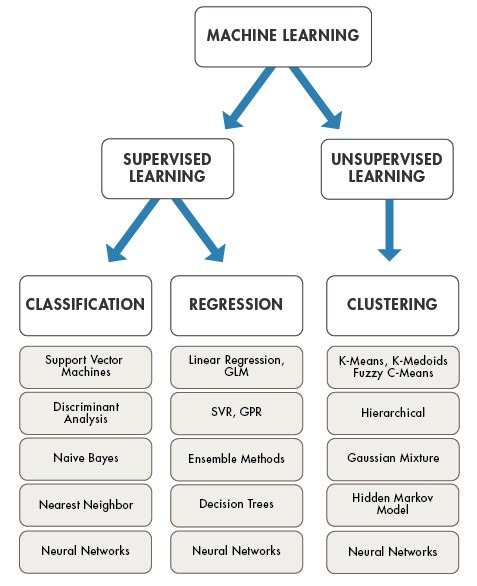
\includegraphics[width=0.7\textwidth]{images/image3.png}
\caption{Overview of machine learning method categories : supervised learning (classification and regression), unsupervised learning (clustering and dimensionality reduction), and reinforcement learning (policy optimization).}
\label{fig:overview_machine_learning_method_categories}
\end{figure}

\subsubsection{Supervised Learning}

In supervised learning, algorithms are trained using labeled datasets where the ``ground truth'' or correct output is already known. In the context of geographic assignment, this process involves feeding the model genetic data associated with individuals of verified geographic origin. The algorithm effectively learns a mapping function that correlates specific genotypes with specific locations. Once this training phase is complete, the model can then be applied to new, unlabelled genetic samples to predict their likely origin with a calculated degree of confidence.

Supervised learning tasks are generally categorized into two main types based on the nature of the target variable. Classification involves assigning input data into discrete, pre-defined categories. For instance, a model might determine whether a sample belongs to the Amazonian population or the Cerrado population based on distinct genetic markers. Regression, on the other hand, is used when the target output is a continuous value. In spatial genetics, regression models can predict precise geographic coordinates (latitude and longitude), offering a continuous gradient of location rather than categorical assignment.

\subsubsection{Unsupervised Learning}

Unsupervised learning differs significantly as the models operate without pre-existing labels or ``correct'' answers. Instead, the algorithm is tasked with identifying inherent structures, patterns, or anomalies within the data itself purely based on the input features. These methods are particularly valuable in conservation for exploratory analysis, such as detecting cryptic population structure or defining management units where prior knowledge is limited or non-existent.

Two primary techniques dominate unsupervised learning in this field. Clustering is the task of grouping a set of objects in such a way that objects in the same group (called a cluster) are more similar to each other than to those in other groups. Dimensionality reduction is the process of reducing the number of random variables under consideration by obtaining a set of principal variables, often to simplify the processing of high-dimensional data. These techniques address the ``curse of dimensionality'' common in genomic studies by condensing massive datasets—such as those containing thousands of Single Nucleotide Polymorphisms (SNPs)—into fewer, informative components that preserve the essential genetic structure while stripping away noise and redundancy.

\subsection{Deep Learning: Specialized Machine Learning}

Deep learning represents a sophisticated subset of machine learning algorithms based on artificial neural networks, which are loosely inspired by the information processing capabilities of the neuron. Unlike ``shallow'' learning models, deep networks are characterized by possessing multiple hidden layers between the input and output. This multi-layered architecture allows them to automatically extract hierarchical patterns from raw data, transforming simple inputs into increasingly abstract representations without the need for manual feature engineering.

The architecture of deep learning models is particularly well-suited to genomic data because the structure of genetic information is inherently hierarchical. At the local level, the initial layers of a network can detect fundamental features such as short DNA motifs or specific combinations of SNPs. These are analogous to detecting edges or textures in image recognition; they represent the basic building blocks of genetic variation.

Moving to an intermediate level of abstraction, deeper layers combine these local features to recognize larger functional units. This might include identifying haplotypes, regulatory elements, or linkage disequilibrium blocks, where the network learns how individual markers interact within a specific genomic region.

Finally, at the global scale, the deepest layers of the model integrate these intermediate patterns to capture broad biological phenomena. This allows the model to detect chromosomal interactions and overarching signals of population structure that emerge from the complex interplay of lower-level genetic features.

\begin{figure}[H]
\centering
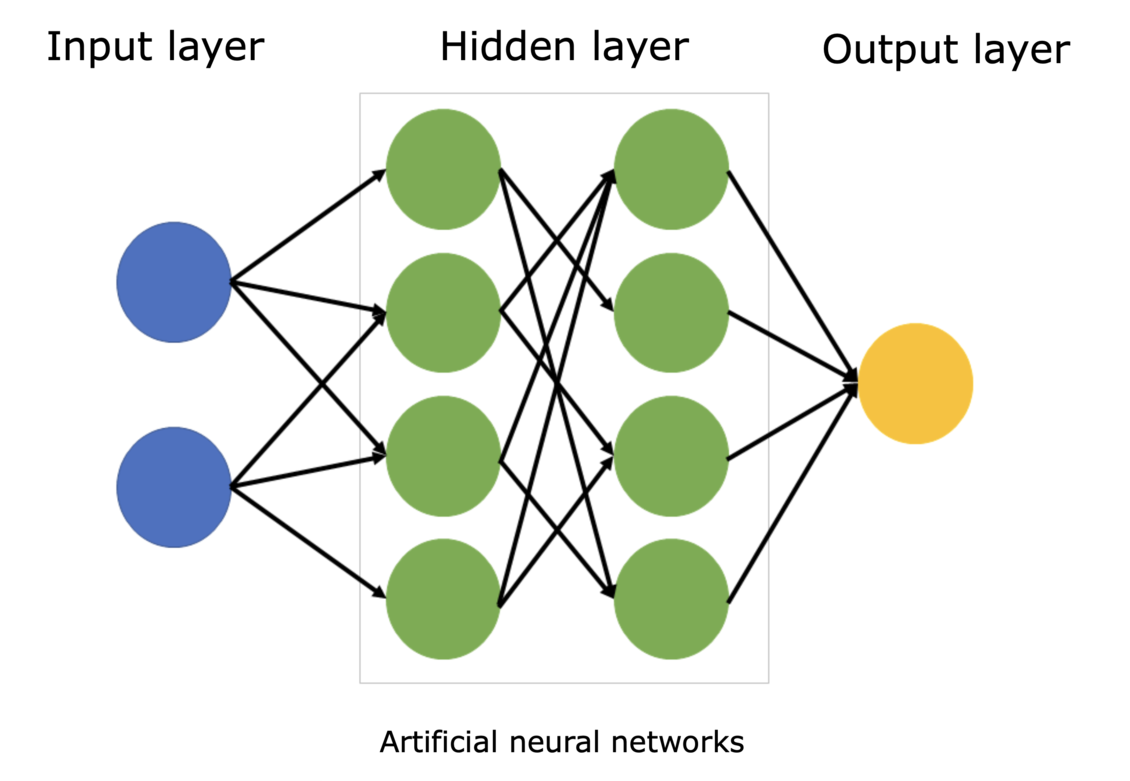
\includegraphics[width=0.7\textwidth]{images/image4.png}
\caption{Simple multilayer perceptron (dense feed-forward neural network) with input, hidden, and output layers.}
\label{fig:simple_multilayer_perceptron_dense_feedforward}
\end{figure}

\subsection{How Machine Learning Models are Trained}

At the heart of machine learning lies the training process: the systematic adjustment of model parameters so that the model can accurately map inputs to outputs. In supervised learning, this means the model is given many examples of input–output pairs. The model generates predictions, compares them to the true labels, and adjusts its internal parameters to minimize error.

Mathematically, this process is expressed as \textbf{loss minimization}. A loss function quantifies the discrepancy between predicted and true outputs. For classification tasks, a common choice is \textbf{cross-entropy loss}, which penalizes incorrect class probabilities. For regression tasks such as predicting coordinates, \textbf{mean squared error (MSE)} is often used. Training involves iterative optimization, most commonly using \textbf{stochastic gradient descent (SGD)} or its variants \cite{kingma2014adam}, which update model parameters in the direction that reduces the loss.

A fundamental concept in evaluating machine learning models is the \textbf{bias–variance tradeoff}, which describes the tension between two competing sources of error that prevent supervised learning algorithms from generalizing beyond their training set.

\textbf{Bias} refers to the error introduced by approximating a real-world problem, which may be extremely complicated, by a much simpler model. This is essentially a systematic error arising from erroneous assumptions in the learning algorithm. This phenomenon is known as \textbf{underfitting}.

\textbf{Variance}, conversely, refers to the model's sensitivity to small fluctuations in the training set. A model with high variance pays too much attention to the specific noise or random idiosyncrasies of the training data, such as genotyping errors or sampling artifacts, rather than the broader population structure. This phenomenon is known as \textbf{overfitting}: the model models the training data too well, effectively memorizing it, but consequently performs poorly when tasked with predicting the origin of new, unseen individuals.

Effective ML requires striking a balance: models should be flexible enough to capture complex relationships in data but not so flexible that they lose predictive power on unseen examples. Techniques such as \textbf{cross-validation}, \textbf{regularization} \cite{srivastava2014dropout} (penalizing overly complex models), and \textbf{early stopping} (halting training before overfitting occurs) are standard strategies to achieve this balance.

\subsubsection{Convolutional and Recurrent Neural Networks}

Before the dominance of transformers, two neural architectures,\textbf{convolutional neural networks (CNNs)} and \textbf{recurrent neural networks (RNNs)}, played a central role in applying deep learning to spatial and sequential data.

\textbf{Convolutional Neural Networks (CNNs)} \cite{krizhevsky2012imagenet} CNNs were originally developed for image analysis, but their ability to detect local patterns has made them highly relevant for genomics. A CNN applies small filters (convolutions) that slide across the input sequence, capturing motifs such as conserved DNA subsequences. Multiple convolutional layers allow the network to combine simple motifs into increasingly complex features. CNNs are computationally efficient and effective at recognizing spatially local but position-independent features, making them well suited to analyzing DNA or protein sequences.

\begin{figure}[H]
\centering
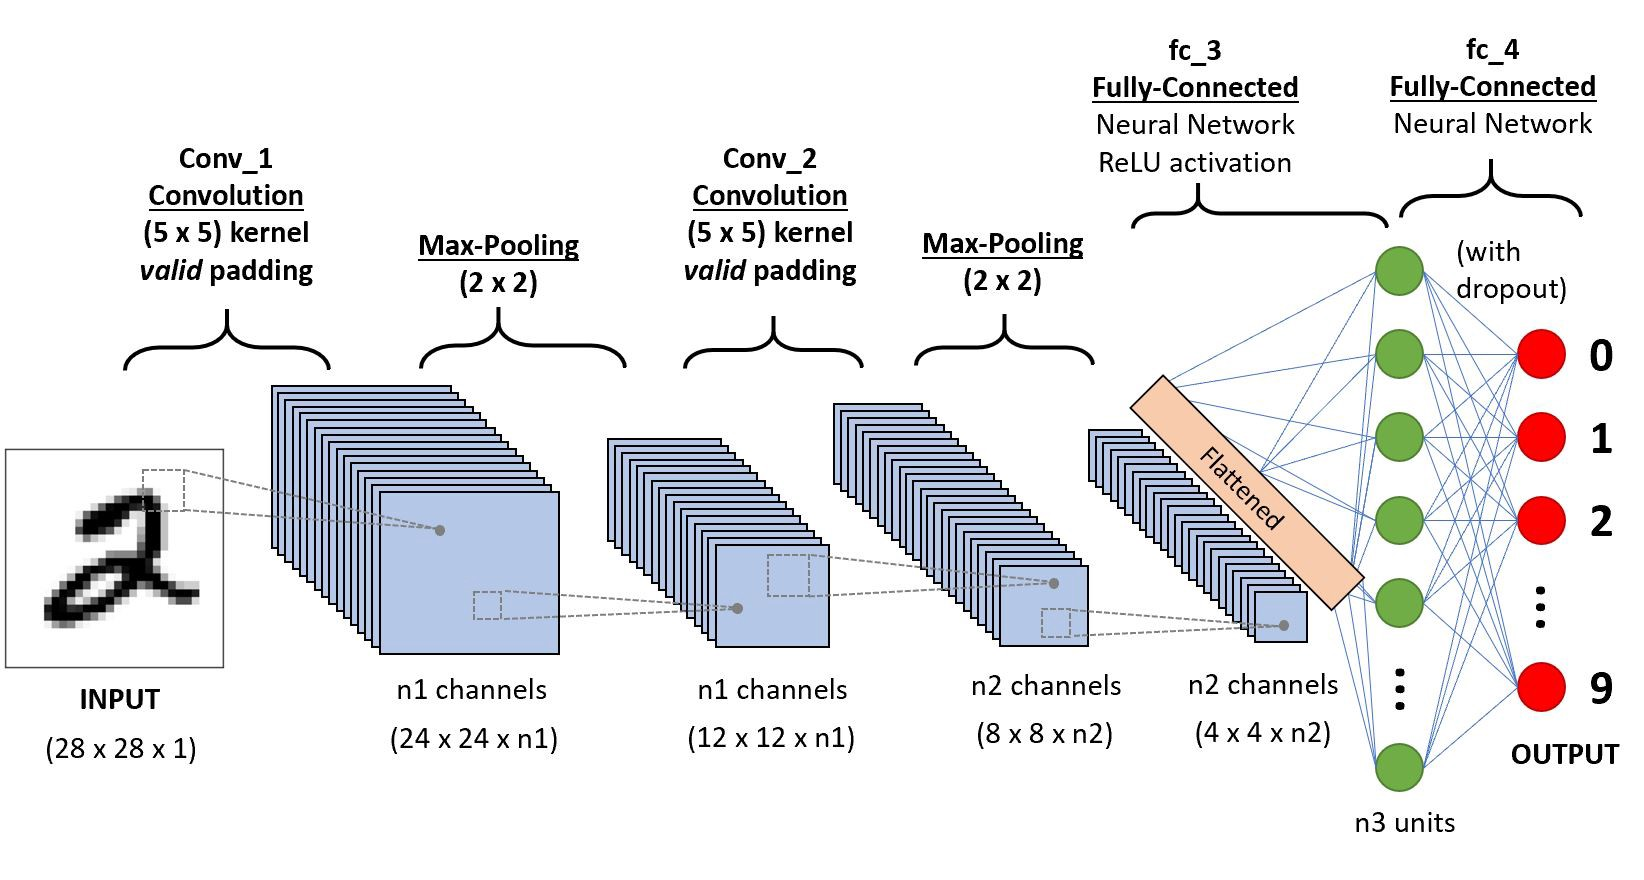
\includegraphics[width=0.9\textwidth]{images/image6.png}
\caption{Convolutional neural network architecture showing feature extraction through convolution and pooling layers, followed by fully connected layers.}
\label{fig:convolutional_neural_network_architecture_showing}
\end{figure}

\textbf{Recurrent Neural Networks (RNNs)} RNNs, by contrast, were designed to process sequential data, where the order of elements is important. Variants such as long short-term memory networks (LSTMs) \cite{hochreiter1997long} and gated recurrent units (GRUs) improve the ability to capture long-range dependencies by mitigating the vanishing gradient problem that limited early RNNs. RNNs have been applied to tasks like splice site prediction and identifying coding regions in DNA.

Both CNNs and RNNs demonstrated the value of deep learning for biological sequence analysis. However, they also had limitations: CNNs struggle to model long-range dependencies, while RNNs are computationally expensive for very long sequences. These shortcomings paved the way for the \textbf{transformer architecture} \cite{vaswani2017attention}, which uses attention mechanisms to capture both local and long-range relationships more efficiently.

\begin{figure}[H]
\centering
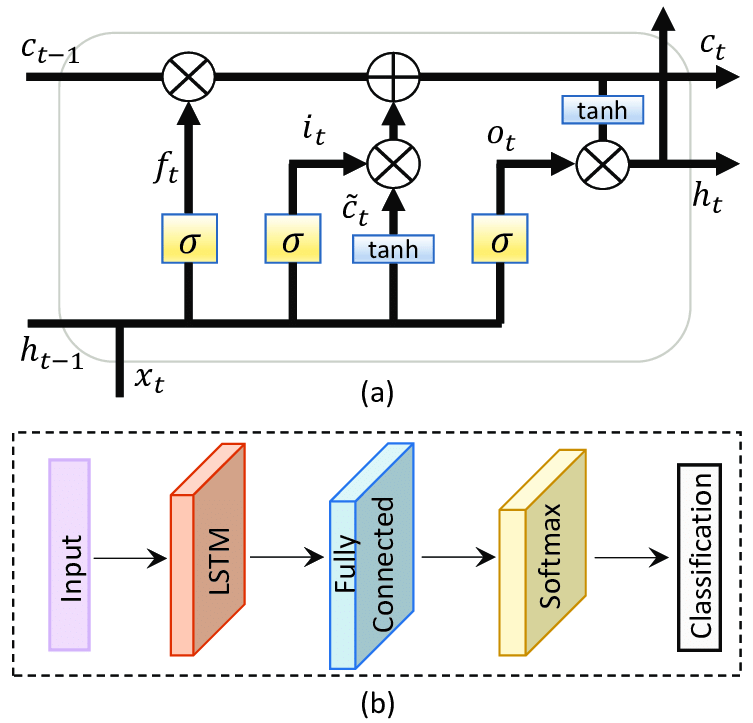
\includegraphics[width=0.6\textwidth]{images/image2.png}
\caption{Structure of an LSTM cell : inputs, forget/input/output gates, cell state, and hidden state flows.}
\label{fig:structure_lstm_cell__inputs}
\end{figure}

\subsection{Challenges and Limitations}

Despite their promise, the application of machine learning methods in conservation genomics introduces a new set of challenges that must be carefully managed.

\subsubsection{Data Requirements}

One of the most significant hurdles is the reliance on data quantity and quality. Most machine learning approaches, particularly deep learning, are data-hungry and require large training datasets to statistically discern signal from noise. In conservation contexts, obtaining high-quality genomic data with reliable geographic labels for rare or elusive species can be logistically difficult and expensive.

\subsubsection{Interpretability}

A major criticism of advanced ML models is their lack of transparency. While traditional statistical methods offer clear coefficients and p-values, complex models, especially deep neural networks, can behave as black boxes. This makes it difficult to understand exactly which genetic features or SNPs are driving the predictions, complicating the biological interpretation of results.

\subsubsection{Computational Costs}

The computational burden of training sophisticated models is non-trivial. Unlike traditional summary statistics that can often be calculated on a standard laptop, training large ML models often demands significant high-performance computing (HPC) resources, including specialized Graphics Processing Units (GPUs). This requirement can limit accessibility for researchers in resource-constrained settings or those lacking technical infrastructure.

\subsubsection{Validation}

Finally, rigorous validation protocols are essential to ensure model reliability. Because ML algorithms are powerful enough to memorize noise, proper techniques such as k-fold cross-validation and the use of independent test sets are critical. Without these safeguards, models may appear highly accurate during training but fail to generalize to new data, falling to the overfitting problems previously described.

\section{Genomic Foundation Models and Transfer Learning}

Recent developments in genomic machine learning have introduced foundation models, which are large-scale pre-trained architectures designed to capture universal features of DNA sequences across species. These models—such as \textbf{DNABERT-2} \cite{zhou2024dnabert} and the \textbf{Nucleotide Transformer} (Dalla-Torre et al., 2025) \cite{dallatorre2025nucleotide}—represent a paradigm shift in the field. Their goal is to learn rich, generalizable representations of nucleotide sequences that can be transferred to diverse downstream tasks, from variant effect prediction to motif discovery, often with minimal fine-tuning data.

\subsection{Why Transformers?}

The shift to transformer architectures is central to this breakthrough. Classical deep learning approaches in genomics, such as convolutional neural networks (CNNs) and recurrent neural networks (RNNs), were powerful but limited. CNNs excel at detecting short sequence motifs. RNNs, while sequentially aware, suffer from vanishing gradients and limited ability to capture dependencies spanning thousands of bases.

Transformers, in contrast, use self-attention mechanisms \cite{vaswani2017attention} that allow the model to directly compute relationships between any pair of positions in a sequence, regardless of distance. This means that a transformer can simultaneously learn short motifs and long-range dependencies. The architecture scales efficiently with parallel computation, enabling training on billions of tokens; something infeasible with older deep learning models. In effect, transformers provide a unified architecture that can model both local and global genomic signals, making them particularly suited to DNA, where both motifs and long-distance regulatory effects are key.

\subsection{Pretraining Tasks and Representations}

Foundation models in genomics rely on \textbf{self-supervised pretraining}, which uses the genome itself as a training signal. DNABERT-2, for example, adapts the \textbf{masked language modeling (MLM)} task from natural language processing: random nucleotides or spans of nucleotides are masked, and the model learns to predict them from context. This forces the model to build a contextual understanding of DNA ``syntax" and ``semantics," capturing motif distributions, codon usage, and structural patterns without requiring labeled data.

The \textbf{Nucleotide Transformer} takes this further, applying MLM across thousands of genomes from diverse species, effectively teaching the model both species-specific features and conserved elements. Pretraining at this scale produces embeddings—vector representations of DNA sequences—that encode structural, functional, and evolutionary information. These embeddings can then be transferred to downstream tasks such as promoter recognition, enhancer classification, splice site detection, or even cross-species generalization tasks, with fine-tuning requiring only modest amounts of labeled data.

\subsection{Impact and Results}

The results have been striking. Both DNABERT-2 and the Nucleotide Transformer achieve state-of-the-art performance across a wide range of genomic benchmarks. DNABERT-2, for instance, outperforms classical CNNs and RNNs on promoter prediction, transcription factor binding site recognition, and splice site identification, often by large margins \cite{zhou2024dnabert}. Similarly, the Nucleotide Transformer has shown that pretraining across many species enables cross-species transfer, where a model trained on non-human genomes can still perform strongly on human tasks \cite{dallatorre2025nucleotide}.


\begin{figure}[H]
\centering
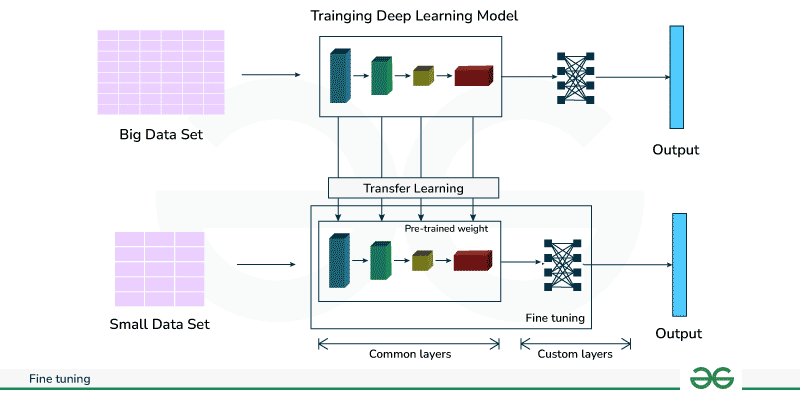
\includegraphics[width=0.9\textwidth]{images/image1.png}
\caption{Illustration of transfer learning and fine-tuning : a pre-trained base model's shared layers are reused, while task-specific layers are added and trained on the target dataset. Understanding Fine-Tuning of Large Language Models (LLMs) : Instruction Tuning and Beyond (Medium, 2023).}
\label{fig:illustration_transfer_learning_and_finetuning}
\end{figure}
